\input{configuration}

\title{Lecture 29 --- Scheduling in Linux }

\author{Jeff Zarnett \\ \small \texttt{jzarnett@uwaterloo.ca}}
\institute{Department of Electrical and Computer Engineering \\
  University of Waterloo}
\date{\today}


\begin{document}

\begin{frame}
  \titlepage

 \end{frame}
 
 
\begin{frame}
\frametitle{Linux}

Linux has two scheduling modes: Real-Time and Non-Real-Time (or perhaps we should call that the ``normal'' one). 

It is not necessary to use the real-time scheduler, strictly speaking. 

If the real-time scheduler is used, the system can still have non-real-time threads which will be scheduled according to the normal scheduler routine.

\end{frame}

\begin{frame}
\frametitle{Linux Real-Time Scheduler}

The Linux scheduler operates based on \alert{scheduling classes}.

There are three classes into which priorities can be assigned:

\begin{itemize}
	\item \texttt{SCHED\_FIFO}: First-In, First-Out Real-Time threads
	\item \texttt{SCHED\_RR}: Round-Robin Real-Time threads
	\item \texttt{SCHED\_OTHER}: Other (non-real-time) threads.
\end{itemize}


In each class, threads may have different priorities relative to one another. 

Lower numbers indicate higher priorities. 

Real-time priorities are in the range [0-99] and the other priorities are [100-139].

\end{frame}

\begin{frame}
\frametitle{Linux Real-Time Scheduler}

The rules for \texttt{SCHED\_FIFO}:

\begin{enumerate}
	\item The system will only interrupt a FIFO thread if one of the following is true:
	\begin{enumerate}
		\item Another FIFO thread of higher priority becomes ready.
		\item The current FIFO thread gets blocked (e.g., on I/O).
		\item The current FIFO thread yields the CPU with \texttt{sched\_yield}.
	\end{enumerate}
	\item If a FIFO thread is interrupted, it is placed in the queue associated with its priority.
	\item If a FIFO thread becomes ready and that thread has higher priority than the currently-executing thread, the currently-executing thread is preempted in favour of the highest priority ready FIFO thread. If two or more threads are at the highest priority, the one that has been waiting the longest is chosen.
\end{enumerate}


\end{frame}

\begin{frame}
\frametitle{Linux Real-Time Scheduler}

The policy is the same for Round-Robin real-time scheduling, except time slicing is implemented. 

If a Round-Robin thread has executed for a full time slice it is suspended and the scheduler will select a real-time thread of equal or higher priority.

It could certainly be the same thread, but is not necessarily. 

\end{frame}

\begin{frame}
\frametitle{Linux Real-Time Scheduler}

\begin{center}
	\includegraphics[width=0.75\textwidth]{images/linux-rts.png}
\end{center}

One of the threads in the \texttt{SCHED\_OTHER} category can execute only if there are no threads in the Round-Robin or FIFO queues that are ready at the moment.


\end{frame}

\begin{frame}
\frametitle{Linux Non-Real-Time Schedulers}

In Linux 2.4 and earlier the Linux kernel used something like the traditional algorithm. 

Then they introduced a scheduling algorithm that was commonly called the $O(1)$ scheduler, because it executed in constant time ($O(1)$). 

Big improvement over the previous scheduling algorithm ($O(n)$).

It also worked a lot better for SMP systems, because it introduced processor affinity and load balancing. 

Since version 2.6.23 of the kernel, however, a new scheduling algorithm has replaced the $O(1)$ scheduler; it is called the \alert{Completely Fair Scheduler} (CFS).


\end{frame}

\begin{frame}
\frametitle{Problems with the Traditional Scheduler}

The traditional UNIX scheduler fell down on a couple of fronts. 

It was not very good at handling very large numbers of processes.

$O(n)$ algorithm, so its performance got worse as more processes appeared. 

It also had significant difficulty with SMP systems due to its design:

\begin{enumerate}
	\item A single run queue;
	\item A single run queue lock; and
	\item An inability to pre-empt running processes.
\end{enumerate}

\end{frame}

\begin{frame}
\frametitle{Problems with the Traditional Scheduler}

The single run queue means a task can and will be scheduled on any processor (good for load balancing), but there is no implementation of processor affinity. 

Thus, a task running on CPU-0 could be easily reassigned to CPU-1 resulting in lots of cache misses.

\end{frame}

\begin{frame}
\frametitle{Problems with the Traditional Scheduler}

The single run queue lock means there is one mutual exclusion construct protecting manipulation of the run queue. 

Thus, when one processor wants to modify it (enqueueing or dequeueing a task, for example), all other processors have to wait.

This can take non-trivial time as an $O(n)$ operation for large values of $n$.


Thus, processors may be waiting for something to do.

\end{frame}

\begin{frame}
\frametitle{Problems with the Traditional Scheduler}

Finally, pre-emption was not possible. 

Lower priority tasks would continue to execute while higher priority tasks wait. 

Only something getting blocked, a time slice expiration, or an interrupt might cause the scheduler to re-evaluate what process should run next.


\end{frame}

\begin{frame}[fragile]
\frametitle{The $O(1)$ Scheduler}

So now that we know the problem with the traditional scheduler, we can see how the $O(1)$ scheduler is designed to address these problems. 

The kernel would maintain two data structures for the processor in the system.

\begin{verbatim}
struct prio_array {
  int nr_active; /* number of tasks in this array */
  unsigned long bitmap[BITMAP_SIZE]; /* priority bitmap */
  struct list_head queue[MAX_PRIO]; /* priority queues */
}
\end{verbatim}

There is one queue for each priority level; \texttt{MAX\_PRIO} (140) is both the highest priority and the number of queues. 

\end{frame}

\begin{frame}
\frametitle{The $O(1)$ Scheduler}

Initially, there are no tasks in any queues and all the bits in the bitmap are zero. 

If a process is created and enters the ready queue, it is put in the queue corresponding to its priority value. 

If that queue was previously empty, then its bit in the bitmap is set to 1 to indicate that queue is no longer empty.


\end{frame}

\begin{frame}
\frametitle{The $O(1)$ Scheduler}


\begin{center}
	\includegraphics[width=0.85\textwidth]{images/linux-o1-struct.png}
\end{center}

\end{frame}

\begin{frame}
\frametitle{The $O(1)$ Scheduler}

If a process does not complete its full time slice before it is preempted, then it goes back in the ready queue. 

If it does run to the end of the time slice, it is placed in the expired queue. 

All scheduling takes place from the active queues. 

The highest priority queue is chosen; if there are multiple tasks in that queue, they are scheduled in Round-Robin fashion. 

This continues until the active queue structure is empty. 

When that happens, the active and expired queues change places, and execution (scheduling) continues.


\end{frame}

\begin{frame}
\frametitle{The $O(1)$ Scheduler}

Part of the difficulty with the $O(1)$ scheduler is that it does not provide very good performance for interactive processes.

These are the ones you work with on your desktop computer. 

Given that the Linux folks always claim that this year or next year is ``the year of the Linux desktop'' (... still waiting for that) a new scheduler was needed. 

Hence, the relatively rapid replacement with the Completely Fair Scheduler.

\end{frame}

\begin{frame}
\frametitle{The CFS}

The CFS, written by Ingo Moln\'ar, is not $O(1)$, unfortunately. 

It uses a red-black tree to model the ready queue, where processes are inserted based on a linear ordering of execution time. 

The leftmost group in this tree is therefore the task that has spent the least amount of time executing and that is what will be scheduled next. 

Because a red-black tree remains balanced, the time to access the leftmost group will be $O($ln$(n))$.

Caching could be used to make access to the next task faster.


\end{frame}

\begin{frame}
\frametitle{The CFS}

If a task gets blocked it will not end up in the queue again. 

If it reaches the end of a timeslice or gets preempted, then it will be inserted into the tree with its updated execution time.

This is very likely not the same place it was taken from (which might require rebalancing the tree (a $O($ln$(n))$ operation).


\end{frame}

\begin{frame}
\frametitle{CFS Red-Black Tree}

\begin{center}
	\includegraphics[width=0.75\textwidth]{images/cfs.png}
\end{center}


\end{frame}

\begin{frame}
\frametitle{The CFS}

Rather than using a strict rule, the CFS scheduler assigns a proportion of CPU processing time to each task based on the nice value. 

A nice value may be in the range -20 to +19 (lower priority is still higher priority).

The CFS does not use a particular length of time slice, but has a \alert{target latency}.

This is an interval of time in which all ready tasks should get to run at least once. 

The CPU time is then doled out based on the targeted latency. 

There are usually default and minimum values, but targeted latency can increase if there is a big increase in the number of tasks to be executed.

\end{frame}

\begin{frame}
\frametitle{The \texttt{vruntime}}

The linear ordering of execution time, called \texttt{vruntime} in the earlier diagram, is also called the \alert{virtual run time}.

 This is a way of keeping track of how much time a task has been executing. 
 
 As with a lot of history keeping, there is a decay factor so that more recent history is more highly weighed in the calculation. 
 
 Higher priority processes' history decays faster; lower priority processes' history decays more slowly. 
 

\end{frame}

\begin{frame}
\frametitle{Virtual Run Time}

For tasks at a normal priority (nice value of zero), the virtual run time equals the physical run time. 

If the physical run time is, say, 50~ms, a process with a nice value of 0 will have a virtual runtime of 50. 

If the process has a positive nice value, the virtual runtime will be larger than 50; if a negative nice value, the virtual runtime will be less than 50.

\end{frame}



\begin{frame}
\frametitle{Virtual Run Time}

Tasks that spend a lot of time using the CPU will, under this system, normally get a lower priority than a task that spends a lot of time waiting for I/O.

So a process that is user-interactive and waiting for user input will get to execute fairly quickly.

This makes the system seem responsive to the user. Which users, of course, like.

\end{frame}

\begin{frame}
\frametitle{CFS: Group Scheduling}

Another thing that is noteworthy in the CFS is the addition of group scheduling. 

We may designate a number of processes as belonging to a group. 

This is useful when a process spawns lots of threads or lots of new processes. 

Instead of treating every thread or process totally equally, a multithreaded program's threads can all be pooled; the group is equal to other processes. 

Within the group, the scheduler will try to treat the threads or processes fairly.

\end{frame}




\begin{frame}
\frametitle{A Decade of Wasted Cores}

2016: researchers exposed serious problems in the scheduler. 

The authors found four significant bugs in Linux multicore scheduling such that there were threads waiting to run even when cores were sitting idle. 

Performance degradation is in the range of 13-24\%, but may be as much as 138 times when looking at some corner cases. 

\end{frame}



\begin{frame}
\frametitle{All Roads Lead to Rome}

There are four different problems but they all cause the same behaviour. \\
\quad Cores are left idle when runnable threads are waiting to execute. 

If it is brief, it is not a problem.

Moving a thread takes some ``effort'' on the part of the scheduler.\\
\quad It may be better to leave it alone. 

But if that thread is waiting an unreasonably long time (in the few hundred milliseconds) then it is a problem.

\end{frame}



\begin{frame}
\frametitle{Be Fair to Everyone}

Recall from earlier the completely fair scheduler we have discussed. 

There will be multiple run queues, one for each core. 

If CPU 0 has 1 low priority thread and CPU 1 has 3 high priority threads, high priority threads will run less than the low priority thread. 

Linux will periodically try to keep the queues balanced.

\end{frame}



\begin{frame}
\frametitle{Do What You Must}

Load balancing is expensive and will run periodically but not often.\\
\quad A completely idle core will result in emergency load balancing.

Load balancing is just look at how busy each of the cores is and move things from the most busy to the least busy core, right?

That oversimplifies the solution because it does not consider cache locality or non-uniform memory access.

\end{frame}



\begin{frame}
\frametitle{Multiple Groups}

Thus, above the level of each core is a larger unit, a scheduling domain. 

Scheduling domains are configured by what hardware they have in common.

\begin{center}
	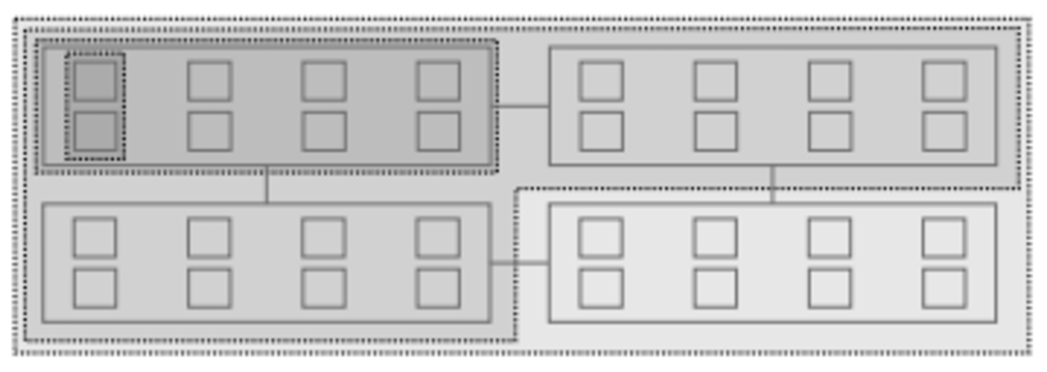
\includegraphics[width=0.7\textwidth]{images/wastedcores.png}\\
\end{center}

\end{frame}



\begin{frame}
\frametitle{The Four Bugs}

So what are the four bugs that caused this problem?
\begin{enumerate}
	\item The group imbalance bug
	\item The scheduling group construction bug
	\item The overload on wakeup bug
	\item The missing scheduling domains bug
\end{enumerate}

\end{frame}



\begin{frame}
\frametitle{The Group Imbalance Bug}

Cores would steal work from other cores if the average load of the victim scheduling group is higher than the average load of the one doing the stealing. 

But averages can be misleading! 

The fix is to use the minimum load of the group, meaning the load of the least loaded core of the group. 

This means cores will steal more often, but this is better than leaving them idle. 

This can result in a 13\% decrease in the runtime of \texttt{make}.

\end{frame}



\begin{frame}
\frametitle{Scheduling Group Construction}

The Linux \texttt{taskset} command allows applications to be pinned to specific cores. 

If the groups are two hops apart, the load balancing thread might not steal them. 

This is because all groups are constructed from the perspective of core 0. 

If load balancing is running on core 31 it might not steal from a neighbour.\\
\quad It thinks it is too far away because it is two hops from core 0.

\end{frame}



\begin{frame}
\frametitle{Overload on Wakeup}

We have already discussed the idea of processor affinity, but sometimes, too much of a good thing is a problem. 

If a thread goes to sleep on group 1, when it and it gets unblocked later by some other thread, the scheduler will try to put it on one of the cores in group 1... 

Even if other groups are not busy! 

This will reduce the number of cache misses, sure, but it means sometimes a thread gets in a queue that's busy rather than one that's free.

\end{frame}




\begin{frame}
\frametitle{Missing Scheduling Domains}

The last bug appears to have been caused by an error during refactoring. 

When a core was removed and re-added, an important function was no longer invoked.

This could cause all threads of an application to run on a single core instead of all of them. 

\end{frame}



\begin{frame}
\frametitle{Scheduling is Hard}

In conclusion: scheduling is by no means a solved problem. 

A simple scheduling algorithm that worked reasonably well in a single core environment was not adequate to the multiple core world. 

Averages can be misleading...\\
\quad And optimizations sometimes do more harm than good. 

\end{frame}

\end{document}

